\chapter{Resultados}
\label{chapter:resultados}

A técnica desenvolvida neste trabalho de graduação foi avaliada a fim de verificar a qualidade do rastreamento obtido e o tempo de execução da técnica, visando o seu uso em aplicações de realidade aumentada. Os experimentos foram executados em um computador equipado com um processador Core i7-3770 3.4 GHz da Intel com 4GB de memória RAM e placa de vídeo GeForce GTS 450 com suporte a CUDA (versão 5.0). O teste em vídeo foi feito utilizando diferentes filmagens, com diferentes quantidades de quadros. Todas as filmagens tem resolução de 320 por 240 \emph{pixels} e tiveram como objetivo rastrear um cubo parado enquanto se fazia movimentos com a câmera utilizada na filmagem.

Foram feitos dois tipos de teste: um de desempenho, que compara o tempo médio para a execução do algoritmo em cada quadro, e o teste de qualidade do rastreamento, que indica, através de um resultado numérico, o quão próxima a pose encontrada está dos pontos extraídos da imagem.

No teste de desempenho foi medido o tempo, em milésimos de segundos, que o algoritmo leva para executar as etapas que permitem o rastreamento (obtenção dos pontos de forte gradiente, escolha das hipóteses, cálculo da pose). Não foi considerado o tempo de obtenção dos quadros a partir da câmera e de renderização do modelo na tela do computador, pois isso é bastante dependente dos respectivos \emph{drivers} de entrada e saída. Neste teste também foi feita uma comparação da velocidade do algoritmo utilizado nesse trabalho (utilizando tanto a implementação em CPU como a implementação em GPU) com o algoritmo de escolha de hipóteses baseado na distância até a amostra do modelo \cite{mestradochico}. O ideal é que cada quadro seja computado em pelo menos 33 milésimos de segundo, o que em termos de quantidade de \emph{frames} por segundo é algo em torno de 30 FPS, que é aproximadamente o limiar humano de percepção de movimento quadro a quadro.

No teste de qualidade foi utilizado como métrica o erro de reprojeção da pose encontrada após a minimização utilizando o algoritmo de Levenberg-Marquardt. Como foi dito anteriormente, o erro de reprojeção é a média das distâncias de cada hipótese de ponto com sua amostra correspondente do modelo utilizando a pose obtida após a minimização. Os resultados do teste de qualidade são independentes da capacidade de processamento da máquina utilizada, portanto também é indiferente se o algoritmo foi executado em GPU ou CPU. No teste aqui apresentado a qualidade do algoritmo será comparada com uma técnica baseada em arestas com múltiplas hipóteses na qual a hipótese mais próxima da amostra sempre é escolhida \cite{mestradochico}.

\section{Qualidade do rastreamento}

Para testar a qualidade do rastreamento o principal ponto a se considerar é o erro de reprojeção da pose. Este tipo de métrica é utilizada em diversos trabalhos relacionados na literatura.

Os dados da \figref{qualidade_cubo_real} mostram a variação do erro de reprojeção (eixo vertical) no decorrer do rastreamento de um cubo. A linha vermelha indica o rastreamento utilizando a técnica descrita neste trabalho, enquanto que a linha verde indica um rastreamento baseado em aresta sem a utilização da clusterização \emph{k-means}. A partir do \emph{frame} 350 há um crescimento no erro de reprojeção em ambos os rastreamentos. Isso foi devido a uma movimentação rápida da câmera durante a gravação do experimento. Após esse movimento na câmera o modelo renderizado passou a não corresponder com o objeto rastreado (veja \figref{brusco_350}). O experimento que utilizou a clusterização, no entanto, conseguiu rapidamente chegar a uma pose mais próxima do objeto enquanto que a abordagem tradicional permaneceu distante até o fim do experimento. Isso pode ser evidenciado ao analisar o gráfico no \emph{frame} 600, onde há um pico no erro de reprojeção, e comparar com a \figref{sequencia_cubo_real}, em que claramente pode-se perceber que que o modelo renderizado pelo \emph{edge-based} está muito distante do objeto rastreado.

\begin{figure}[!ht]
\centering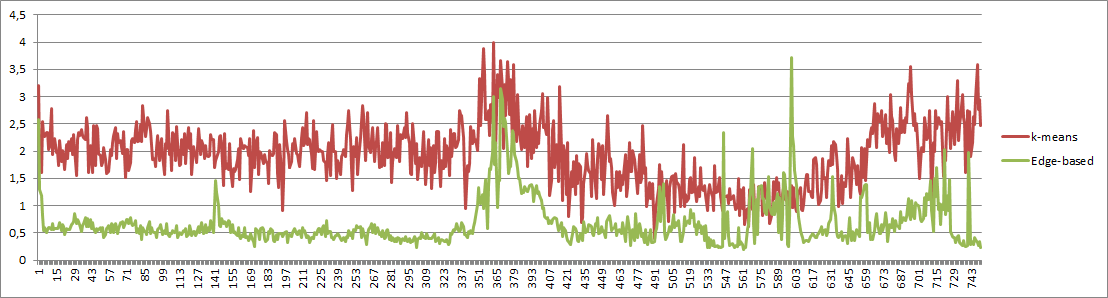
\includegraphics[width=\textwidth]{monografia/qualidade_cubo_real}
\caption{Gráfico de qualidade do rastreamento de um cubo.}
\label{qualidade_cubo_real}
\end{figure}

\begin{figure}[!ht]
\centering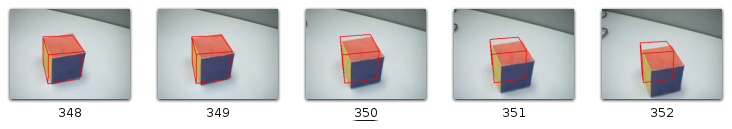
\includegraphics[width=\textwidth]{monografia/brusco_350}
\caption{Sequência de \emph{frames} mostrando como estava o modelo antes e como ficou depois do \emph{frame} 350.}
\label{brusco_350}
\end{figure}

Foi observado nos testes que apesar das vantagens teóricas para a escolha da melhor hipótese, a técnica discutida apresenta bastante instabilidade na escolha da pose. Mesmo quando a câmera está em repouso, as poses calculadas em dois \emph{frames} consecutivos podem mudar bruscamente. Isso também pode ser visto no gráfico da \figref{qualidade_cubo_real} no que diz respeito à instabilidade no erro de reprojeção da linha vermelha. Observe que enquanto a linha verde tem poucas variações no decorrer do tempo, a linha vermelha tem muitas variações, no decorrer de todo o experimento.

Apesar do que foi mostrado no gráfico acima, ao se analisar o rastreamento quadro a quadro, pode ser visto que em determinado momento (a partir do \emph{frame} 500) o rastreamento utilizando a técnica baseada em arestas tradicional calcula uma pose bastante diferente do objeto rastreado, mesmo que o erro de reprojeção continue pequeno. Por outro lado, a técnica desenvolvida neste trabalho apresenta erros de reprojeção maiores, porém a pose se aproxima bastante do objeto. Na \figref{sequencia_cubo_real} é possível observar a sequência de \emph{frames} nos dois casos.

\begin{figure}[!t]
\centering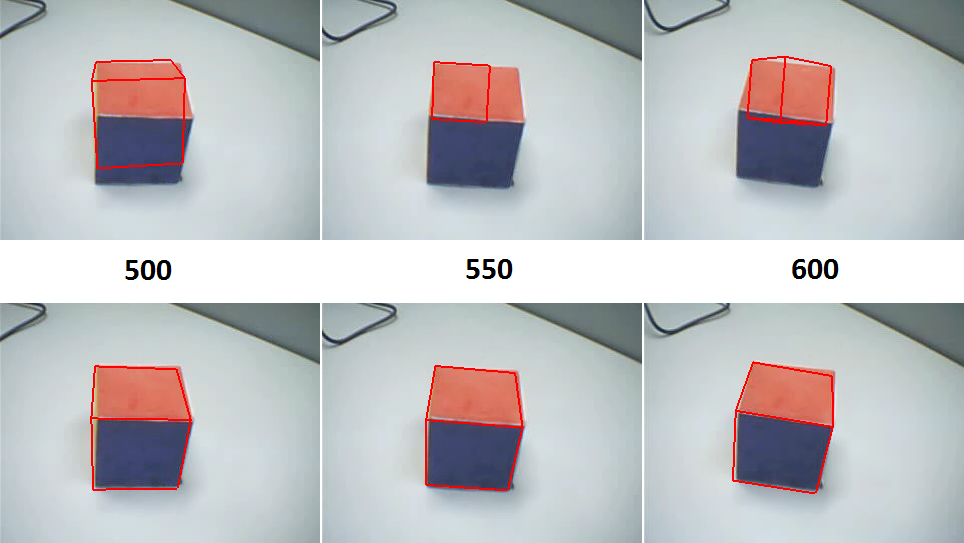
\includegraphics[width=\textwidth]{monografia/sequencia_cubo_real}
\caption{Sequência de imagens comparando as duas técnicas de rastreamento. A imagem mostra tanto o cubo a ser rastreado como também o modelo sendo renderizado. O sequência de baixo é resultado do algoritmo que utiliza a clusterização \emph{k-means} e a de cima é resultado do rastreamento baseado em arestas sem a utilização da técnica.}
\label{sequencia_cubo_real}
\end{figure}

Foi notado nos experimentos que o algoritmo não apresenta melhora significativa na qualidade do rastreamento comparado com outras técnicas já existentes. O fato das amostras escolhidas serem as mais colineares possíveis torna o rastreamento bastante instável, pois não muito raro as amostras que formam o conjunto mais colinear se distanciam bastante da aresta do modelo, chegando em alguns casos a uma posição quase que perpendicular a que deveria realmente ser escolhida. O algoritmo encontra muita dificuldade em manter a pose escolhida e é possível perceber isso ao analisar o vídeo. Por outro lado, notou-se que um ponto forte da técnica é a facilidade em encontrar a pose correta quando o modelo está bastante distante do real. Nesses casos ela obteve os melhores resultados. Foi realizado outro experimento em que a câmera era movimentada constantemente com o objetivo de testar se o rastreamento consegue se recuperar com facilidade. Assim como na \figref{qualidade_cubo_real}, a \figref{qualidade_celine_boa} mostra a variação do erro de reprojeção (eixo vertical) no decorrer do tempo (eixo horizontal) e compara a técnica implementada neste trabalho (linha vermelha) com uma técnica de rastreamento baseado em arestas sem utilizar o \emph{k-means} (linha verde). Com o algoritmo deste trabalho a pose sempre volta a rastrear o objeto, apesar de todas as movimentações; o mesmo não acontece com o algoritmo tradicional. No final do experimento percebe-se que o erro de reprojeção da técnica que utiliza o \emph{k-means} já é menor que o erro do rastreamento tradicional. Neste momento a técnica \emph{edge-based} não conseguiu mais rastrear o objeto enquanto que a abordagem utilizada neste trabalho conseguiu encontrar novamente uma pose próxima ao objeto rastreado.

\begin{figure}[!ht]
\centering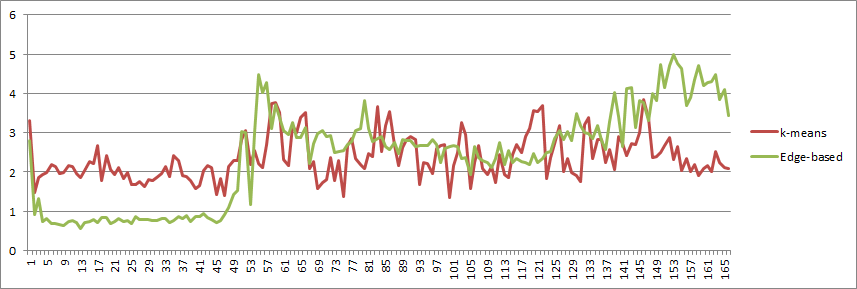
\includegraphics[width=\textwidth]{monografia/qualidade_celine_boa}
\caption{Gráfico comparativo de qualidade em um teste em que são feitos vários movimentos com a câmera}
\label{qualidade_celine_boa}
\end{figure}

\section{Desempenho}

No teste de desempenho é avaliado o tempo, em milésimos de segundo, no qual o algoritmo foi executado. Esse tipo de teste depende bastante da máquina utilizada, mas é importante discuti-lo para se fazer uma comparação relativa entre as técnicas apresentadas. O vídeo de entrada utilizado nos três testes é uma sequência de 751 \emph{frames} de um cubo parado enquanto que a câmera faz alguns movimentos. Foi feito o teste utilizando os algoritmos de múltiplas poses de câmera rodando tanto em GPU quanto em CPU, como também foi utilizado um algoritmo de hipótese única de câmera para efeitos de comparação. A \figref{performance} mostra um gráfico comparativo de desempenho das três simulações. O eixo horizontal mostra os \emph{frames} do vídeo e o eixo vertical mostra o tempo de execução de cada \emph{frame} em milissegundos. Como é um teste de tempo de execução, quanto menor o valor, melhor o resultado. Deseja-se executar o algoritmo em um tempo menor que 33 milésimos de segundo, por \emph{frame}, para que a execução seja considerada em tempo real.

\begin{figure}[!ht]
\centering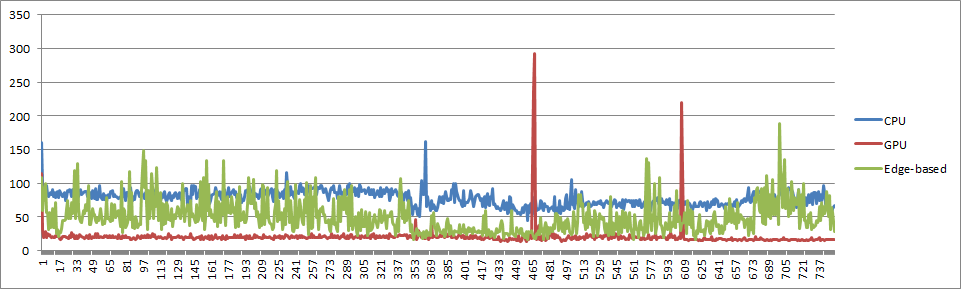
\includegraphics[width=\textwidth]{monografia/performance}
\caption{Gráfico comparativo da performance do algoritmo em CPU e em GPU. Também é mostrado um rastreamento sem utilizar o algoritmo para efeitos de comparação. A linha pontilhada mostra o limite para que a execução seja considerada em tempo real.}
\label{performance}
\end{figure}

A \figref{performance} mostra um gráfico comparativo do desempenho do algoritmo executado tanto em CPU (linha azul) quanto em GPU (linha vermelha). Para efeitos de comparação com técnicas já existentes, também foi feito o mesmo teste com uma abordagem baseada em aresta tradicional (linha verde). O eixo vertical indica o tempo de execução do rastreamento em cada \emph{frame} (eixo horizontal) e a linha preta pontilhada é o limiar para que a execução seja considerada em tempo real. Como essa é uma medida de tempo, quanto menor o valor do eixo vertical, melhor o desempenho. No gráfico pode-se observar que o uso de múltiplas hipóteses de pose juntamente com a clusterização \emph{k-means} aumenta bastante o tempo de execução do algoritmo. Apesar disso, o mesmo algoritmo implementado em CUDA apresenta resultados melhores do que a implementação em CPU da técnica de pose única, sendo inclusive o único cuja execução do experimento pode ser considerada em tempo real, pois praticamente todos os \emph{frames} são executado em menos de 33 milissegundos (linha preta do gráfico).
